
\subsubsection{Mengenoperationen und Teilmengen}
Vergleicht man die Elemente der Mengen \(\mathbb{Z}\) und \(\mathbb{N}\), so stellt man fest, dass alle Elemente von \(\mathbb{N}\) auch in \(\mathbb{Z}\) enthalten sind. Man sagt dann, dass \(\mathbb{N}\) eine Teilmenge von \(\mathbb{Z}\) ist:

\begin{definition}{Teilmenge}{teilmenge}
    Eine Menge \(A\) heisst \textit{Teilmenge} einer Menge \(B\), wenn alle Elemente von \(A\) auch in der Menge \(B\) liegen.

    Schreibweise:
    \[
        A \subset B
    \]

    \begin{center}
        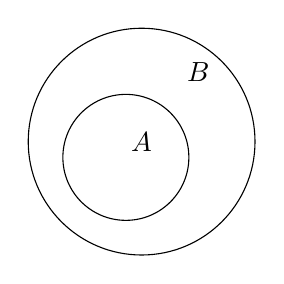
\begin{tikzpicture}[scale=0.8]
            \draw (0,0) circle (1.8);
            \draw (-0.25,-0.25) circle (1.0);
            \node at (0,0) {\(A\)};
            \node at (0.9,1.1) {\(B\)};
        \end{tikzpicture}
    \end{center}
\end{definition}

Bemerkung: Ist \(A\) keine Teilmenge von \(B\), schreibt man
\[
    A \not\subset B.
\]

\textbf{Beispiel:}
\[
    \mathbb{Z} \subset \mathbb{R}.
\]

\begin{definition}{Schnittmenge}{schnittmenge}
    Die \textit{Schnittmenge} der Mengen \(A\) und \(B\) ist diejenige Menge, die alle Elemente enthält, welche in \(A\) und in \(B\) enthalten sind.

    Schreibweise für Schnittmengen:
    \[
        A \cap B
    \]

    Es gilt:
    \[
        A \cap B = \{x \mid x \in A \text{ und } x \in B\}.
    \]

    \begin{center}
        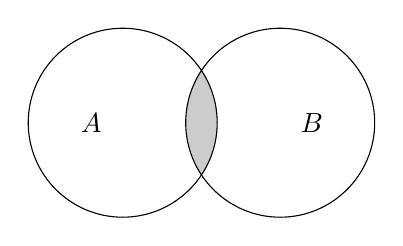
\begin{tikzpicture}
            \begin{scope}
                \clip (-1,0) circle (1.2);
                \fill[gray!40] (1,0) circle (1.2);
            \end{scope}
            \draw (-1,0) circle (1.2);
            \draw (1,0) circle (1.2);
            \node at (-1.4,0) {\(A\)};
            \node at (1.4,0) {\(B\)};
        \end{tikzpicture}
    \end{center}
\end{definition}

\textbf{Beispiel einer Schnittmenge:}
\[
    \{\text{Primzahlen}\}
    \cap
    \{\text{natürliche Zahlen kleiner als } 10\}
    =
    \{2,3,5,7\}.
\]

\begin{definition}{Vereinigungsmenge}{vereinigungsmenge}
    Die \textit{Vereinigungsmenge} der Mengen \(A\) und \(B\) ist diejenige Menge, die alle Elemente enthält, die in der Menge \(A\) oder \(B\) enthalten sind.

    Schreibweise für Vereinigungsmengen:
    \[
        A \cup B
    \]

    Es gilt:
    \[
        A \cup B = \{x \mid x \in A \text{ oder } x \in B\}.
    \]

    \begin{center}
        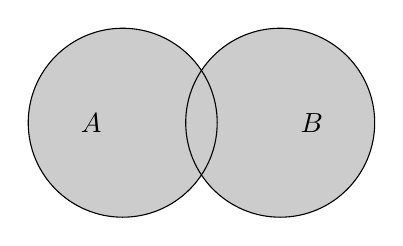
\begin{tikzpicture}
            \fill[gray!40] (-1,0) circle (1.2);
            \fill[gray!40] (1,0) circle (1.2);
            \draw (-1,0) circle (1.2);
            \draw (1,0) circle (1.2);
            \node at (-1.4,0) {\(A\)};
            \node at (1.4,0) {\(B\)};
        \end{tikzpicture}
    \end{center}
\end{definition}

\textbf{Beispiel einer Vereinigungsmenge:}
\[
    \{\text{Teiler von } 6\}
    \cup
    \{x \mid x \in \mathbb{N} \text{ und } 4 < x < 8\}
    =
    \{1,2,3,5,6,7\}.
\]

\begin{definition}{Differenzmenge}{differenzmenge}
    Die \textit{Differenzmenge} der Mengen \(A\) und \(B\) ist diejenige Menge, die alle Elemente enthält, die in der Menge \(A\), aber nicht in der Menge \(B\) enthalten sind.

    Schreibweise für Differenzmengen:
    \[
        A \setminus B
    \]

    Es gilt:
    \[
        A \setminus B
        =
        \{x \mid x \in A \text{ und } x \notin B\}.
    \]

    \begin{center}
        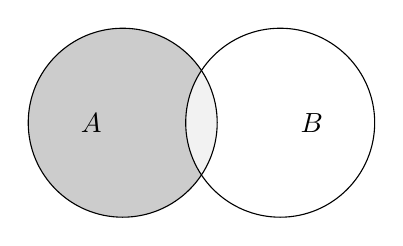
\begin{tikzpicture}
            \begin{scope}
                \clip (-1,0) circle (1.2);
                \fill[gray!40] (-1,0) circle (1.2);
                \fill[gray!10] (1,0) circle (1.2);
            \end{scope}
            \draw (-1,0) circle (1.2);
            \draw (1,0) circle (1.2);
            \node at (-1.4,0) {\(A\)};
            \node at (1.4,0) {\(B\)};
        \end{tikzpicture}
    \end{center}
\end{definition}

\textbf{Beispiel einer Differenzmenge:}
\[
    \{\text{Teiler von } 6\}
    \setminus
    \{\text{Primzahlen}\}
    =
    \{1,6\}.
\]

In Anwendungssituationen wird häufig nur ein beschränkter Bereich der reellen Zahlen betrachtet. Wenn die Variable \(v\) die Schnelligkeit eines Teilchens in \(\mathrm{m/s}\) beschreibt, so ist \(v\) eine reelle Zahl zwischen Null und der Lichtgeschwindigkeit \(c \cong 299'792'458\).

In der Sprache der Mathematik würde man sagen: \(v\) liegt im \textbf{Intervall} \([0,c]\).

\begin{definition}{Intervalle}{intervalle}
    \textbf{Intervalle} sind Mengen von reellen Zahlen zwischen zwei Grenzen. Je nachdem, ob die eckigen Klammern nach innen oder aussen zeigen, gehören die Grenzen zur Menge oder nicht. Für \(a<b\) gilt:
    \[
        \begin{aligned}
            [a,b]                                                & = \{x \in \mathbb{R} \mid a \leq x \leq b\}, \\
            ]a,b[                                                & = \{x \in \mathbb{R} \mid a < x < b\},       \\
            [a,b[   &= \{x \in \mathbb{R} \mid a \leq x < b\},\\
                    ]a,b] & = \{x \in \mathbb{R} \mid a < x \leq b\}.
        \end{aligned}
    \]
\end{definition}

\textbf{Speziell:} Man kann mit der Intervallschreibweise auch unbeschränkte Mengen angeben. Die Menge aller reellen Zahlen, die grösser oder gleich \(5\) sind, wäre zum Beispiel
\[
    M = [5,\infty[.
\]

Analog ist
\[
    ]-\infty,10[
\]
die Menge aller reellen Zahlen, die kleiner als \(10\) sind.

Oder im Extremfall:
\[
    \mathbb{R} = ]-\infty,\infty[.
\]

Merke: Bei \(\infty\) zeigt die Klammer immer gegen aussen.

\begin{bsp}
    {}{}
    \[ [-2, 2 [ \, \cap \, ]0, 3] = ? \]
    \vspace*{5 cm}
\end{bsp}







\clearpage

\begin{ueb}
    {Zu Mengenoperationen und Intervalle}{}
    \begin{enumerate}
        \item Setzen Sie für \(\diamond\) das richtige Zeichen
              \(\left(\in,\notin,\subset,\not\subset\right)\) ein.

              \begin{enumerate}
                  \item \(\mathbb{Z} \diamond \mathbb{Q}\)
                  \item \(\mathbb{Z} \diamond \mathbb{N}\)
                  \item \(-5 \diamond \mathbb{N}\)
                  \item \(-5 \diamond \mathbb{Q}\)
                  \item \(\{2,7\} \diamond \mathbb{N}\)
                  \item \(\{0,\pm1,\pm2,\pm3,\ldots\} \diamond \mathbb{Z}\)
              \end{enumerate}

        \item Gegeben sind die Mengen
              \[
                  A=\{11,13,15,17,18\}
                  \qquad\text{und}\qquad
                  B=\{10,12,13,14,16\}.
              \]
              Bestimmen Sie:

              \begin{enumerate}
                  \item \(A \cup B\)
                  \item \(A \cap B\)
                  \item \(A \setminus B\)
                  \item \(B \setminus A\)
                  \item \((A \setminus B)\cup(B \setminus A)\)
                  \item \((A \cup B)\setminus(A \cap B)\)
              \end{enumerate}

        \item Setzen Sie für \(\diamond\) das richtige Zeichen
              \(\left(\in,\notin,\subset,\not\subset\right)\) ein.

              \begin{enumerate}
                  \item \(b \diamond \{a,b,c,d,e,f\}\)
                  \item \(\{b\} \diamond \{a,b,c,d,e,f\}\)
                  \item \(\{b,d,g\} \diamond \{a,b,c,d,e,f\}\)
                  \item \(g \diamond \{a,b,c,d,e,f\}\)
                  \item \(\{a,b,c,d,e\} \diamond \{a,b,c\}\)
                  \item \(\{b,c,d,e\} \diamond \{b,c,d,e\}\)
              \end{enumerate}

        \item Beurteilen Sie, ob die Aussage wahr oder falsch ist.

              \begin{enumerate}
                  \item \((A \cup B) \subset B\)
                  \item \((A \cap B) \subset B\)
                  \item \(A \subset (A \cup B)\)
                  \item \(A \subset (A \cap B)\)
              \end{enumerate}
        \item Geben Sie die folgenden Mengen als ein Intervall an:

              \begin{enumerate}
                  \item \(A = \{x \in \mathbb{R} \mid -5 < x \leq 3\}\)
                  \item \(B = \{x \in \mathbb{R} \mid 1 < x < 2.5\}\)
                  \item \(C = \{x \in \mathbb{R} \mid x < 1\}\)
                  \item \(D = [-1,5] \cup [4,6[\)
                  \item \(E = [-1,5] \cap [4,6[\)
                  \item \(F = [-2,8] \setminus [5,9]\)
              \end{enumerate}
    \end{enumerate}
\end{ueb}


\emph{Lösungen:}
\begin{enumerate}
    \item
          \begin{enumerate}
              \item \(\mathbb{Z} \subset \mathbb{Q}\)
              \item \(\mathbb{Z} \not\subset \mathbb{N}\)
              \item \(-5 \notin \mathbb{N}\)
              \item \(-5 \in \mathbb{Q}\)
              \item \(\{2,7\} \subset \mathbb{N}\)
              \item \(\{0,\pm1,\pm2,\pm3,\ldots\} \subset \mathbb{Z}\)
          \end{enumerate}

    \item
          \begin{enumerate}
              \item \(A \cup B = \{10,11,12,13,14,15,16,17,18\}\)
              \item \(A \cap B = \{13\}\)
              \item \(A \setminus B = \{11,15,17,18\}\)
              \item \(B \setminus A = \{10,12,14,16\}\)
              \item \((A \setminus B)\cup(B \setminus A) = \{10,11,12,14,15,16,17,18\}\)
              \item \((A \cup B)\setminus(A \cap B) = \{10,11,12,14,15,16,17,18\}\)
          \end{enumerate}

    \item
          \begin{enumerate}
              \item \(b \in \{a,b,c,d,e,f\}\)
              \item \(\{b\} \subset \{a,b,c,d,e,f\}\)
              \item \(\{b,d,g\} \not\subset \{a,b,c,d,e,f\}\)
              \item \(g \notin \{a,b,c,d,e,f\}\)
              \item \(\{a,b,c,d,e\} \not\subset \{a,b,c\}\)
              \item \(\{b,c,d,e\} \subset \{b,c,d,e\}\)
          \end{enumerate}

    \item
          \begin{enumerate}
              \item Falsch.
              \item Wahr.
              \item Wahr.
              \item Falsch.
          \end{enumerate}

    \item
          \begin{enumerate}
              \item \(A = ]-5,3]\)
              \item \(B = ]1,2.5[\)
              \item \(C = ]-\infty,1[\)
              \item \(D = [-1,6[\)
              \item \(E = [4,5]\)
              \item \(F = [-2,5[\)
          \end{enumerate}
\end{enumerate}

\clearpage



